% !TEX root = ../../main.tex


\begin{figure}[!htb]
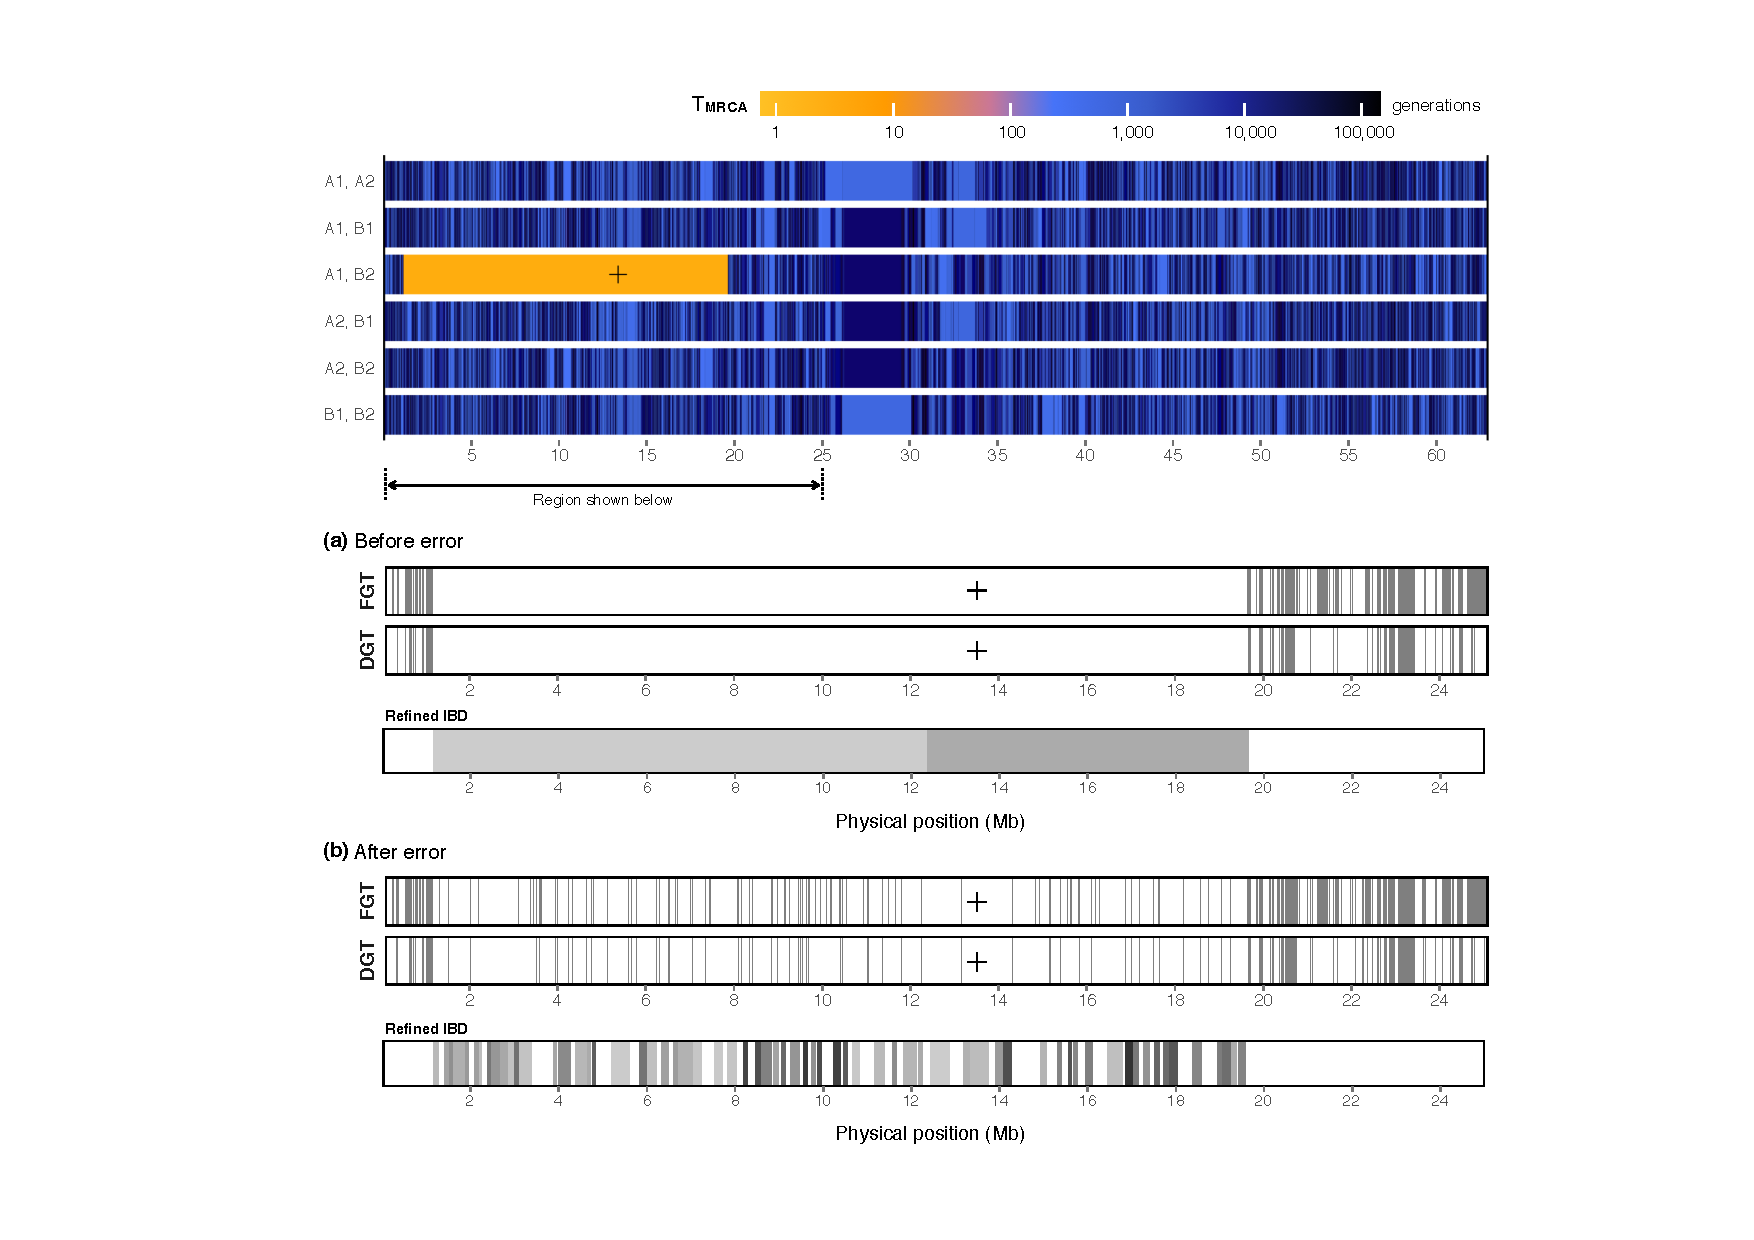
\includegraphics[width=\textwidth]{./img/ch4/full_ibd_error_new}
\Caption{Example of the effect of genotype error on IBD detection}
{One allele and a pair of individuals sharing that allele were randomly selected and the underlying IBD structure for all \n{6} possible pairs of the \n{4} chromosomes was determined from simulation records (\emph{top}).
The figure shows the ``mosaic'' of IBD segments along the sequence of the simulated chromosome; distinguished by the \gls{tmrca}.
The focal shared allele is indicated at the pair of chromosomes sharing that allele (\emph{cross}).
Data were compared before \textbf{(a)} and after \textbf{(b)} the integration of empirically determined genotype error.
In each dataset, the \gls{fgt} and \gls{dgt} were used to detect all breakpoints to the left and right-hand side of the target position.
In addition, the IBD segments reported for the focal pair of haplotypes using the \texttt{Refined\,IBD} method are shown before and after error, where each segment is distinguished by a different colour on grey-scale.
Note that these results were produced on true haplotype data but not phased haplotypes, to highlight the impact of genotype error alone.
Data were simulated using \texttt{msprime} (see \ctref{sec:msprime}).\CorrectLabel}
{fig:full_ibd_error}
\end{figure}
